
\documentclass[%
 reprint,
%superscriptaddress,
%groupedaddress,
%unsortedaddress,
%runinaddress,
%frontmatterverbose, 
%preprint,
%preprintnumbers,
%nofootinbib,
%nobibnotes,
%bibnotes,
 amsmath,amssymb,
 aps,
%pra,
%prb,
%rmp,
%prstab,
%prstper,
%floatfix,
]{revtex4-2}
\usepackage{gensymb}
\usepackage{textcomp}
\usepackage{graphicx}% Include figure files
\usepackage{dcolumn}% Align table columns on decimal point 


\usepackage{bm}% bold math
\usepackage{siunitx}
\sisetup{separate-uncertainty=true}
\usepackage{tabularx}
\usepackage{amssymb}
\usepackage{amsmath}
\usepackage{relsize}
\usepackage{caption}
\usepackage{enumitem}
\usepackage{float}
\usepackage{mhchem}
\usepackage[colorlinks,bookmarks=false,citecolor=blue,linkcolor=blue,urlcolor=blue]{hyperref}
%\usepackage{hyperref}% add hypertext capabilities
%\usepackage[mathlines]{lineno}% Enable numbering of text and display math
%\linenumbers\relax % Commence numbering lines

%\usepackage[showframe,%Uncomment any one of the following lines to test 
%%scale=0.7, marginratio={1:1, 2:3}, ignoreall,% default settings
%%text={7in,10in},centering,
%%margin=1.5in,
%%total={6.5in,8.75in}, top=1.2in, left=0.9in, includefoot,
%%height=10in,a5paper,hmargin={3cm,0.8in},
%]{geometry}

\begin{document}

\preprint{APS/123-QED}

\title{Emission Spectra of Hydrogen and\\ Determination of Rydberg's constant}% Force line breaks with \\


\author{Maitrey Sharma}
\email{maitrey.sharma@niser.ac.in}
\affiliation{School of Physical Sciences, National Institute of Science Education and Research, HBNI, Jatni-752050, India}




\date{\today}% It is always \today, today,
             %  but any date may be explicitly specified

\begin{abstract}
In this experiment, we study the phenomena of spectroscopy, more specifically, emission spectroscopy as a means to investigate the behaviour of a matter when it interacts with electromagnetic radiation. We analyse the emission spectrum of atomic hydrogen and obtain the various spectral series and concentrate our attention on Balmer series which lies in the visible spectrum. Balmer series, was discovered through the Balmer formula, devised by Johann Balmer in 1888. He observed the Hydrogen line spectrum in the visible range and made predictions for higher frequency lines. In this experiment we perform the experiment that Balmer did and try to study and verify the Hydrogen spectrum as well as the validity of the formula for energy difference between orbitals. Balmer's efforts were further improved by Niels Bohr and ultimately played a vital role in the development of quantum mechanics. 
\end{abstract}

\keywords{Stokes' Law, Electric force}
\maketitle

%\tableofcontents

\section{\label{sec:level1}Introduction}
    The experiments performed by Sir Isaac Newton in the field of optics in the latter half of seventeenth century opened the path for a new branch of study when he permitted sunlight to pass through a small hole and then through a prism. Newton found that sunlight, is actually made up of a mixture of all the colors of the rainbow (see figure \ref{fig:prism}) which he described by the term \textit{spectrum}. After that, the improvements made by William Hyde Wollaston, and the experiments conducted by Joseph von Fraunhofer during the early 1800s ultimately led to the formation of a more precise and quantitative scientific technique which we today refer to as \textbf{spectroscopy}.
    \begin{figure}
        \centering
        \includegraphics[scale = 0.1]{Figures/Light_dispersion_of_a_mercury-vapor_lamp_with_a_flint_glass_prism_IPNr°0125.jpg}
        \caption{A prism analyses white light by dispersing it into its component colors.}
        \label{fig:prism}
    \end{figure}
    \par
    Spectroscopy, at its core, is the study of the interaction between matter and electromagnetic radiation as a function of the wavelength or frequency of the radiation. And after the advent of quantum mechanics in the twentieth century, spectroscopy became of even immense importance. Historically, the most experiments concerning spectroscopy involved the study of the wavelength dependence of the absorption by gas phase matter of visible light dispersed by a prism. This has now evolved to the precise study of color as generalized from visible light to all bands of the electromagnetic spectrum.
    \par
    The emission spectrum of a chemical element or chemical compound is the spectrum of frequencies of electromagnetic radiation emitted due to an atom or molecule making a transition from a high energy state to a lower energy state. The photon energy of the emitted photon is equal to the energy difference between the two states. There are many possible electron transitions for each atom, and each transition has a specific energy difference. This collection of different transitions, leading to different radiated wavelengths, make up an emission spectrum. As each element's emission spectrum is unique, we can employ the use of spectroscopy to investigate the compositions of an unknown piece of matter. When the elements or their compounds are heated either on a flame or by an electric arc they emit energy in the form of light. Analysis of this light, with the help of a spectroscope gives us a discontinuous spectrum. \textbf{Emission spectroscopy} is a spectroscopic technique which examines the wavelengths of photons emitted by atoms or molecules during their transition from an excited state to a lower energy state. Its development in the nineteenth century and efforts in theoretical explanation of atomic emission spectra eventually led to quantum mechanics.
    \par
    \begin{figure*}
        \centering
        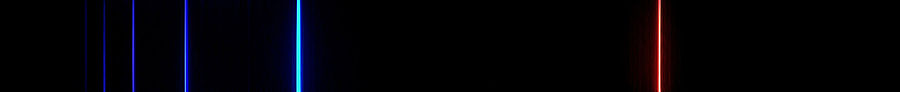
\includegraphics[scale = 0.5]{Figures/900px-Visible_spectrum_of_hydrogen.jpg}
        \caption{The ``visible'' hydrogen emission spectrum lines in the Balmer series. H-alpha is the red line at the right. Four lines (counting from the right) are formally in the visible range. Lines five and six can be seen with the naked eye, but are considered to be ultraviolet as they have wavelengths less than $\SI{400}{\nano \metre}$.}
        \label{fig:balmer}
    \end{figure*}
    Many spectra have been studied in detail and amongst them, the hydrogen emission spectrum which is relatively simple and shows regularity, remains the most intensely studied. The emission spectrum of atomic hydrogen has been divided into a number of spectral series, and the one we will be studying in this experiment is referred to as the \textbf{Balmer series} (see figure \ref{fig:balmer}), which was first discovered by John Balmer in 1885.
    
    

\section{\label{sec:setup}Experimental Setup}
    Before getting to the actual schematics and setup of the experiment to obtain the emission spectra of Hydrogen, we will first concentrate our attention on main equipment used in the experiment, the prism spectrometer (see figure \ref{fig:spectrometer}).
    \begin{figure}
        \centering
        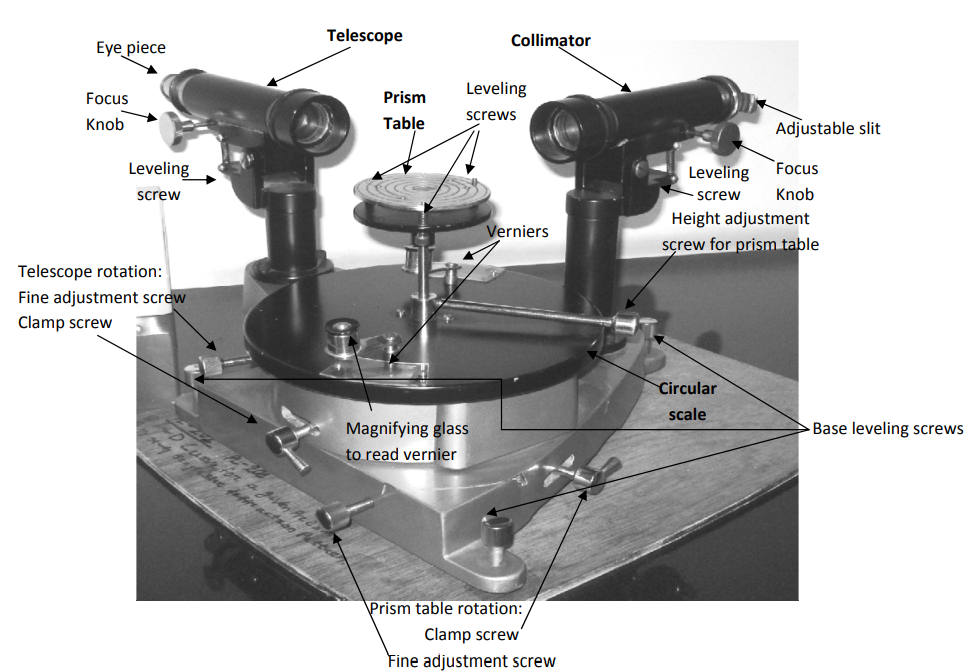
\includegraphics[scale = 0.42]{Figures/spectrometer.png}
        \caption{Different parts of the spectrometer}
        \label{fig:spectrometer}
    \end{figure}
    \par
    The spectrometer is an instrument for studying the optical spectra. Light coming from a source is usually dispersed into its various constituent wavelengths by a dispersive element (prism or grating) and then the resulting spectrum is studied. We will be using a prism spectrometer for our experiment.
    \par
    It consists of a collimator, a telescope, a circular prism table and a graduated circular scale along with two verniers. The collimator holds an aperture at one end that limits the light coming from the source to a narrow rectangular slit. A lens at the other end focuses the image of the slit onto the face of the prism. The telescope magnifies the light dispersed by the prism  and focuses it onto the eyepiece. The angle between the collimator and telescope are read off by the circular scale. The description of each element is discussed below.
    \begin{enumerate}[label=(\roman*)]
        \item \textbf{\textit{Collimator}} ($C$): It consists of a horizontal tube with a converging achromatic lens at one end of the tube and a vertical slit of adjustable width at the other end. The slit can be moved in or out of the tube by a rack and pinion arrangement using the focus knob and its width can be adjusted by turning the screw attached to it. When properly focused, the slit lies in the focal plane of the lens. Thus the collimator provides a parallel beam of light.
        \item \textbf{\textit{Prism table}} ($P$): It is a small circular table and capable of rotation about a vertical axis. It is provided with three leveling screws. A screw attached to the axis of the prism table fixes it with the two verniers and also keep it at a desired height. These two verniers rotate with the table over a circular scale graduated in fraction of a degree. The angle of rotation of the prism table can be recorded by these two verniers.
        \item \textbf{\textbf{Telescope}} ($T$): It is a small astronomical telescope with an achromatic doublet (figure \ref{fig:doublet}) as the objective and the Ramsden type eye-piece (figure \ref{fig:ramsden}). The eye-piece is fitted with cross-wires and slides in a tube which carries the cross-wires. The tube carrying the cross wires in turn, slides in another tube which carries the objective.
        \begin{figure}
            \centering
            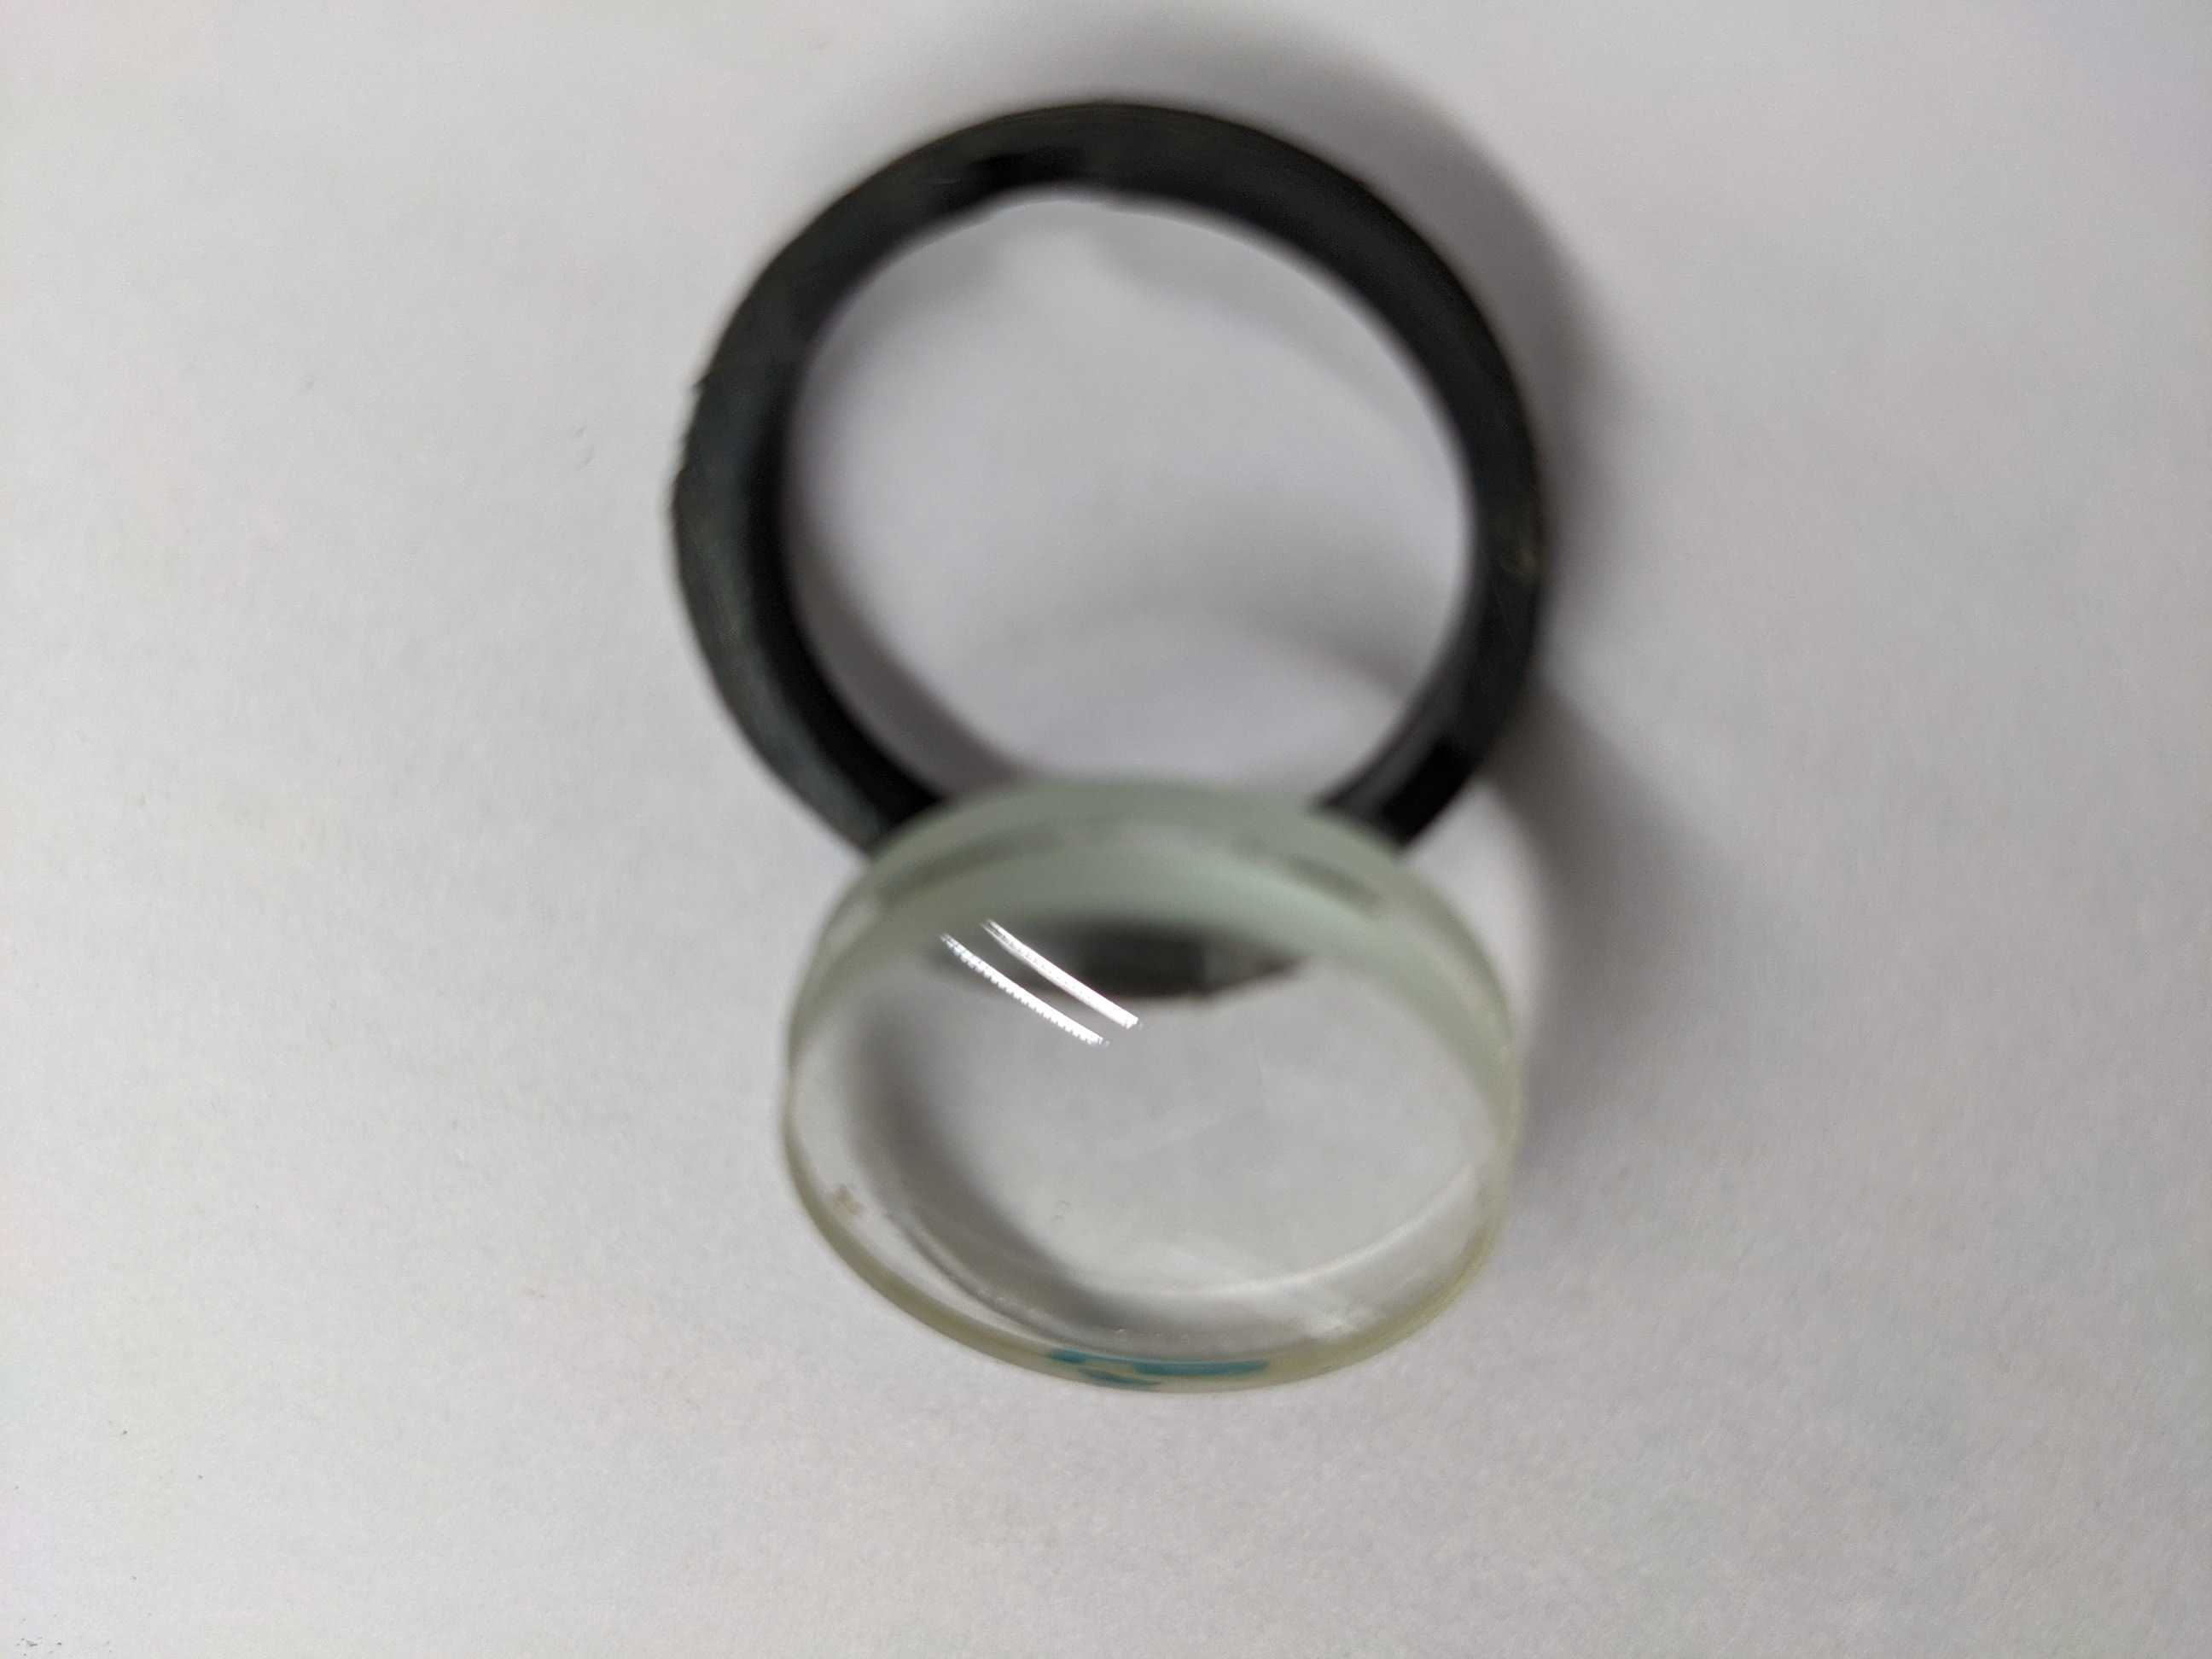
\includegraphics[scale = 0.05]{Figures/PXL_20210913_105948470.jpg}
            \caption{An achromatic doublet which used in the Telescope.}
            \label{fig:doublet}
        \end{figure}
        \begin{figure}
            \centering
            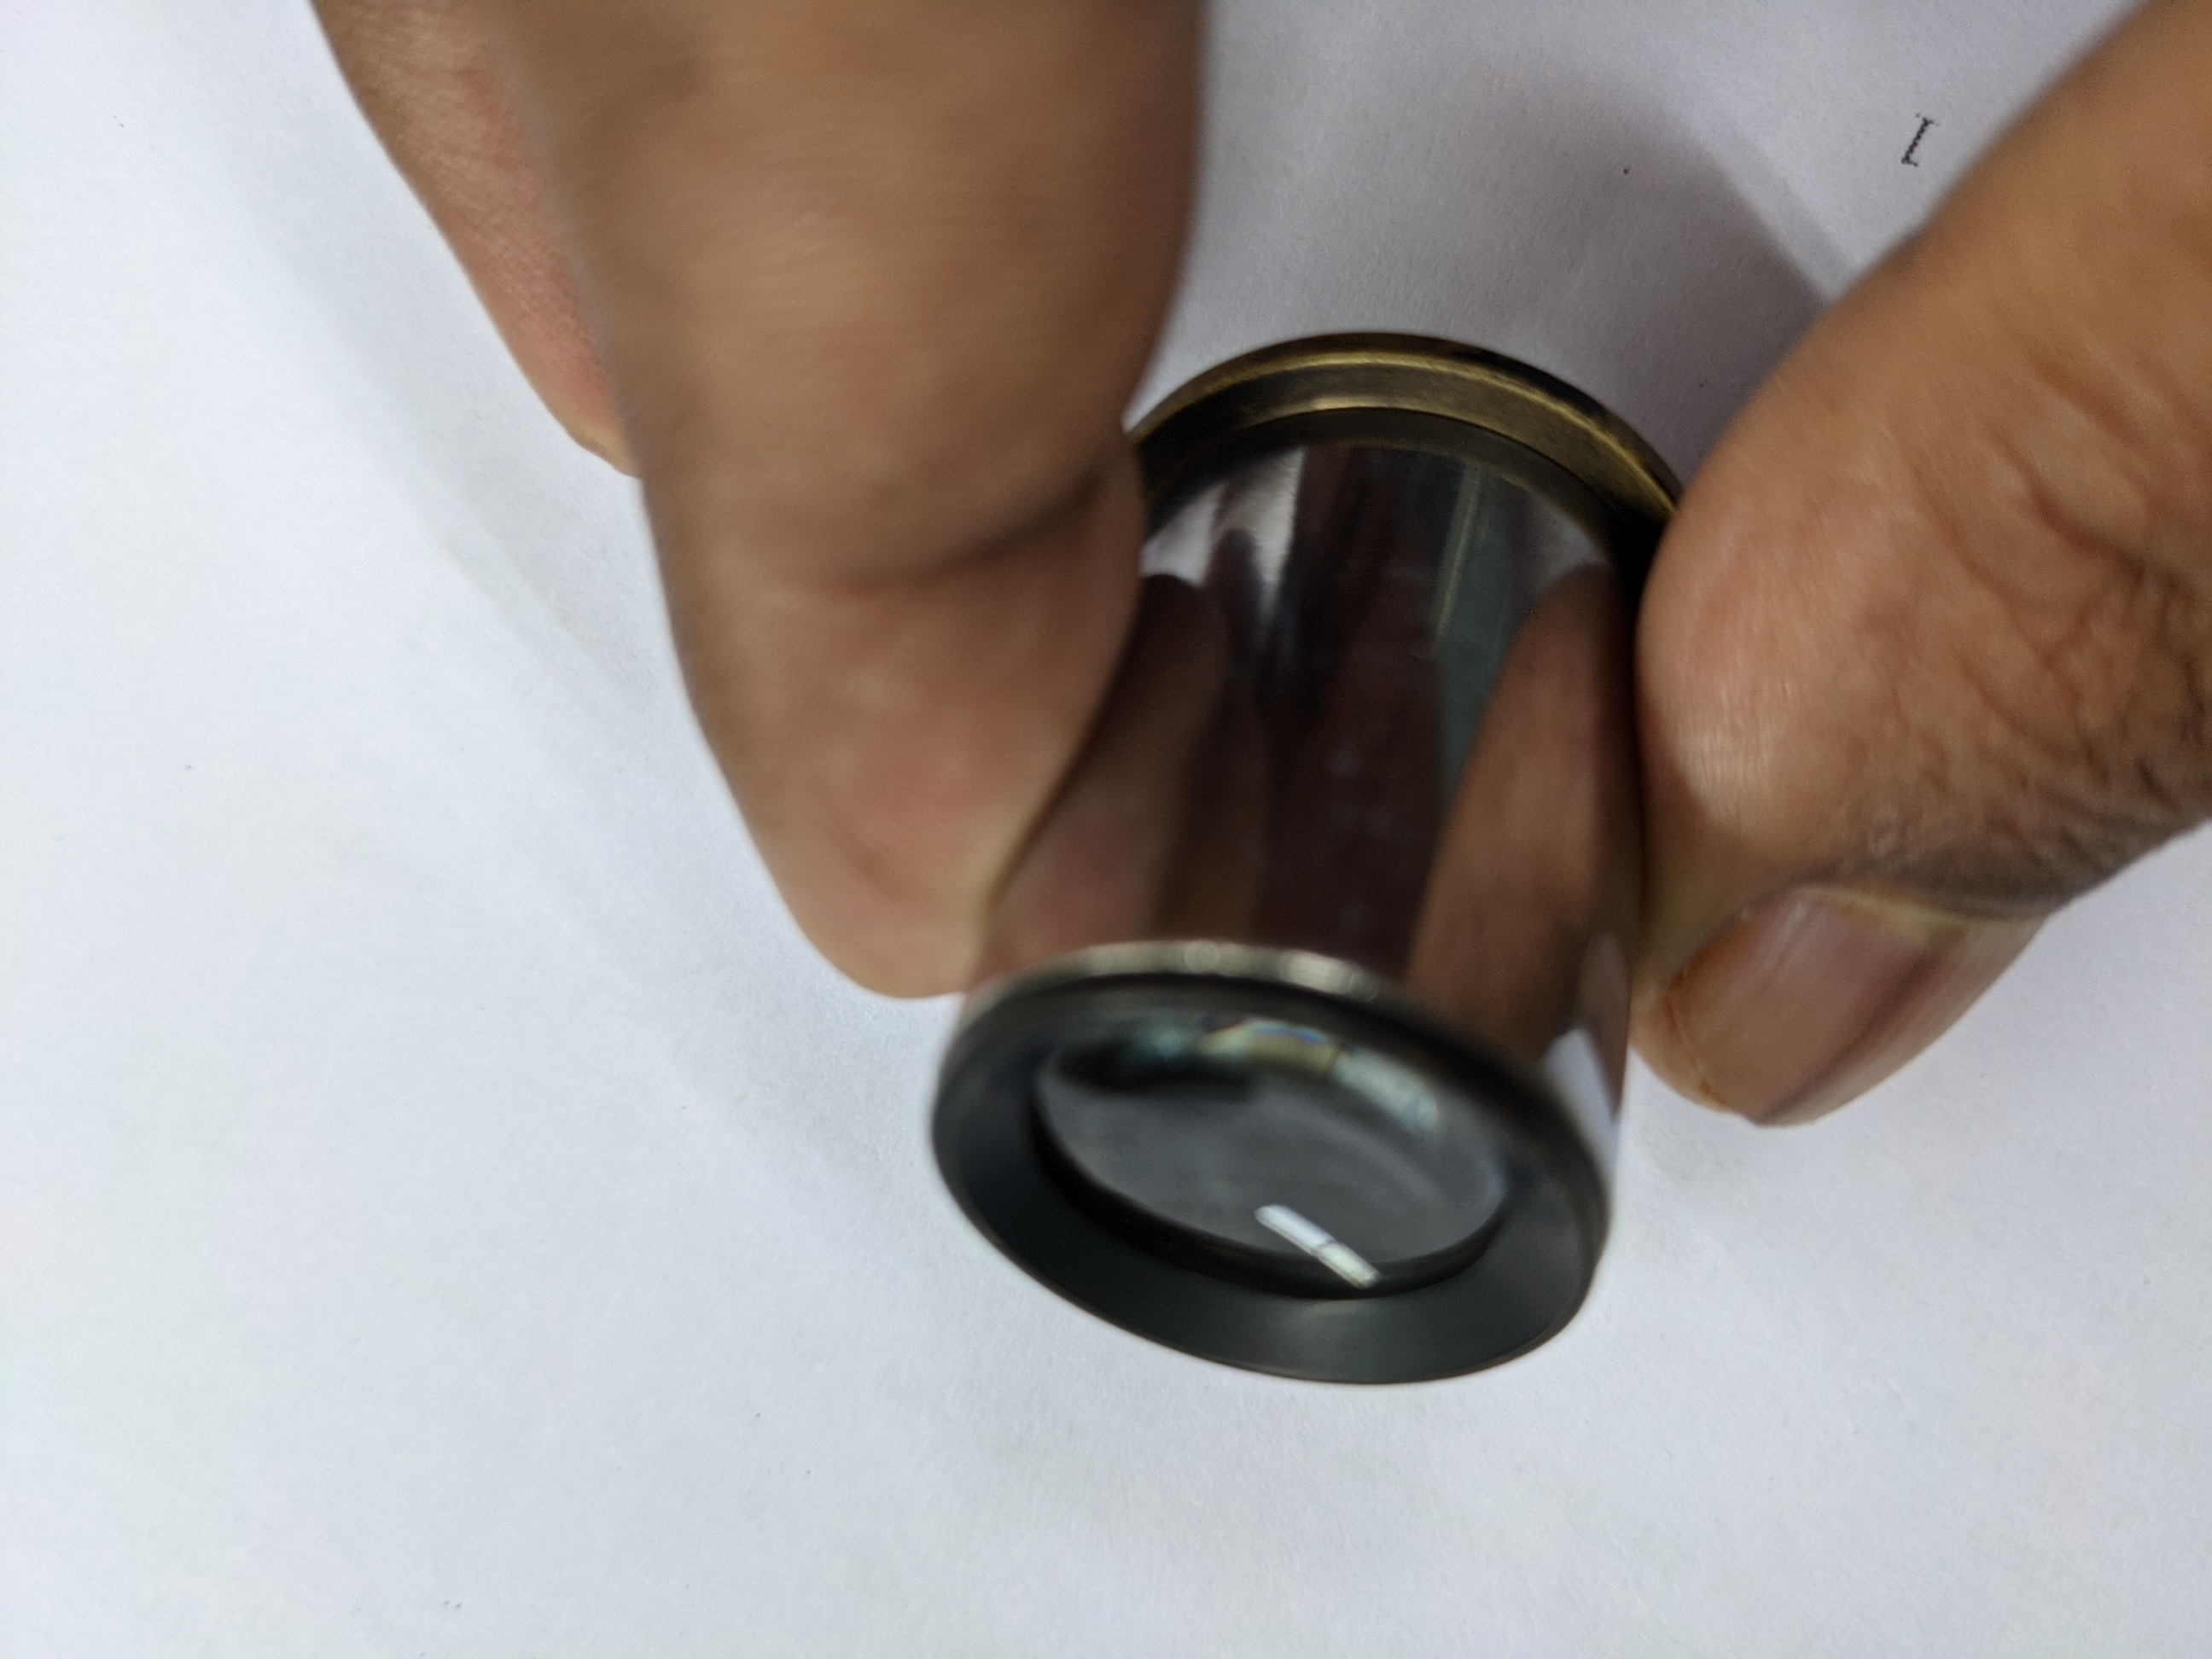
\includegraphics[scale = 0.05]{Figures/PXL_20210913_110035232.jpg}
            \caption{The Ramsden type eye-piece.}
            \label{fig:ramsden}
        \end{figure}
        \item \textbf{\textit{Circular Scale}} ($C.S.$): It is graduated in degrees and coaxial with the axis of rotation of the prism table and the telescope. A separated circular plate mounted co-axially with the circular scale carries two verniers, $V_1$ and $V_2$, 180\degree\ apart.
    \end{enumerate}
    \par
    Before beginning a spectrometer experiment, some essential adjustments should be performed to level the apparatus which are as follows:
    \begin{enumerate}[label=(\roman*)]
        \item \textbf{\textit{Levelling of telescope}}: A spirit level on the telescope tube such that its axis is parallel to that of the telescope. The air bubble of the spirit level is brought halfway towards the centre by first turning the two base leveling screws and then turning the telescope leveling screw. The telescope is then rotated through 180\degree\ and adjust the base and telescope leveling screws. This is repeated until the bubble settles at the centre for both positions of the telescope. After this, the telescope is placed in the line with the collimator and the air bubble of the spirit level is brought at the centre by turning the base leveling screw below the collimator.
        \item \textbf{\textit{Levelling of collimator}}: The spirit level is placed on the collimator along its length and the air bubble of the spirit level is brought at the centre by adjusting the collimator leveling screw provided below the collimator.
        \item \textbf{\textit{Levelling of the prism table}}: The spirit level is placed at the centre of the prism table and parallel to the line joining two of the leveling screws of the prism table and the air bubble of the spirit level is brought at the centre by turning these two screws in the opposite directions. After this, the spirit level is placed perpendicular to the line joining the two screws and bring the bubble at the centre by adjusting the third screw.
        \item \textbf{\textit{Adjusting cross-wires and focusing image}}: The eye-piece is moved inwards or outwards until the cross-wire appears distinct. The image is made very sharp p by turning the focusing knob of the telescope and of the collimator. The image should be made vertical by turning the slit in its own plane, if not already. The width of the slit can be adjusted to get an image of desired intensity. 
        \item \textbf{\textit{Optical levelling of the prism}}: As the bottom face is not exactly perpendicular to the edges, the prism is leveled by the optical method. The slit is illuminated by sodium light and the telescope is placed with its axis making an angle of about 90\degree\ with that of the collimator. The prism on the prism table is placed with its vertex coinciding with that of the table and with one of its faces (faces $AB$ in figure \ref{fig:mindev}) perpendicular to the line joining two of the leveling screws of the prism table. The prism table is rotated till the light reflected from this face $AB$ of the prism enters the telescope and the image is brought at the centre of the field of the telescope by turning the two screws equally in the opposite directions. And finally, the prism table is rotated again till the light reflected from the other face $AC$ of the prism enters the telescope, and bring the image at the centre of the field by turning the third screw of the prism table.
        \begin{figure}
            \centering
            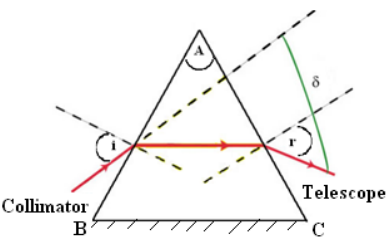
\includegraphics{Figures/mindevlightray.png}
            \caption{Minimum deviation of light ray.}
            \label{fig:mindev}
        \end{figure}
        \item \textbf{\textit{Schuster’s method}}: This method is used to focus the telescope and the collimator for parallel rays within the space available in the dark room. The prism is placed on the spectrometer table as shown in figure (\ref{fig:mindev}). As the angle of deviation for the given prism is 50\degree, the telescope is set at an angle a few degrees greater than this ($\sim 55\degree$). The slit of the spectrometer is illuminated with light from a sodium lamp and the images of the slit are observed through the telescope as it passes through the minimum deviation position. The telescope is locked at an angle a few degrees greater than this position. The prism table is turned away from its minimum deviation position so that apex $A$ moves towards the telescope and a spectral line is brought into the centre of the field of view of the telescope. Then the the prism table is turned to the other side of the minimum deviation position until the same spectral line is again at the centre of the telescopes field of view. We repeat this process until no further adjustment is required.
    \end{enumerate}
    \par
    The setup used in our experiment is shown in figure (\ref{fig:setup}).
    \begin{figure}
        \centering
        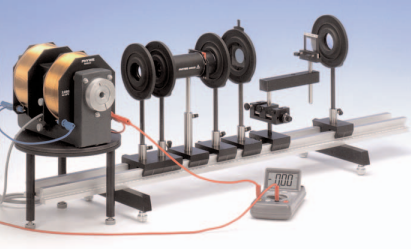
\includegraphics[scale = 1]{Figures/setup.png}
        \caption{Experimental set up with the prism spectrometer to obtain the emission spectra of Hydrogen.}
        \label{fig:setup}
    \end{figure}
    

\section{Theory}
    A hydrogen atom consists of an electron orbiting its nucleus. The electromagnetic force between the electron and the nuclear proton leads to a set of quantum states for the electron, each with its own energy. These states were visualized by the Bohr model of the hydrogen atom as being distinct orbits around the nucleus. Each energy level, or electron shell, or orbit, is designated by an integer, $n$ as shown in the figure (\ref{fig:Hatom}).
    \begin{figure}
        \centering
        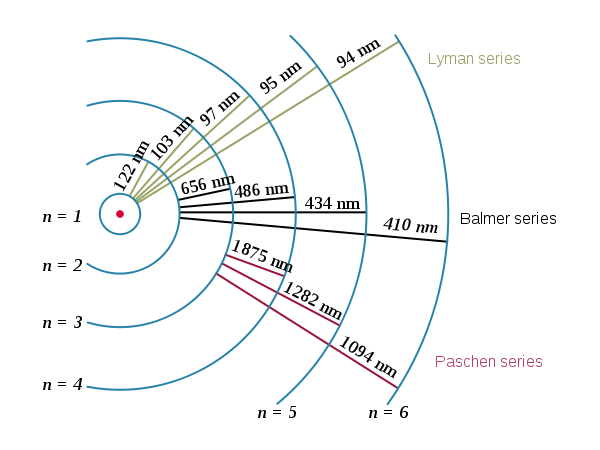
\includegraphics[scale = 0.4]{Figures/600px-Hydrogen_transitions.svg.png}
        \caption{Electron transitions and their resulting wavelengths for hydrogen. Energy levels are not to scale.}
        \label{fig:Hatom}
    \end{figure}
    \par
    Spectral emission occurs when an electron transitions, or jumps, from a higher energy state to a lower energy state. To distinguish the two states, the lower energy state is commonly designated as $m$, and the higher energy state is designated as $n$. The energy of an emitted photon corresponds to the energy difference between the two states. Because the energy of each state is fixed, the energy difference between them is fixed, and the transition will always produce a photon with the same energy.
    \par
    The spectral lines are grouped into series according to $m$. Lines are named sequentially starting from the longest wavelength/lowest frequency of the series, using Greek letters within each series. There are six named series which describe he spectral line emissions of the hydrogen atom and are called \textit{Lyman} ($m = 1$), \textit{Balmer} ($m = 2$), \textit{Paschen} ($m = 3$), \textit{Brackett} ($m = 4$), \textit{Pfund} ($m = 5$) and \textit{Humphreys} ($m = 6$) series. Therefore, the $2 \rightarrow 1$ line is called ``Lyman-alpha'' (Ly-$\alpha$), while the $7 \rightarrow 3$ line is called ``Paschen-delta'' (Pa-$\delta$) (see figure \ref{fig:specseries}).
    \begin{figure*}
        \centering
        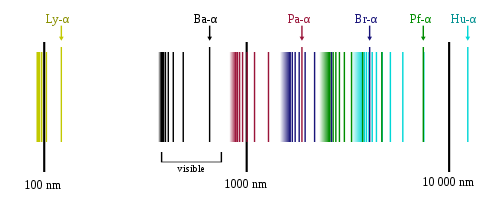
\includegraphics[scale = 0.8]{Figures/500px-Hydrogen_spectrum.svg.png}
        \caption{The spectral series of hydrogen, on a logarithmic scale.}
        \label{fig:specseries}
    \end{figure*}
    \par
    According to Bohr's model, the wavelengths of emitted or absorbed photons, is given by the \textbf{Rydberg formula}:
    \begin{equation}
        \dfrac{1}{\lambda} = Z^2 R_{\infty} \Bigg(\dfrac{1}{m^2} - \dfrac{1}{n^2} \Bigg)
    \end{equation}
    where, $Z$ is the atomic number, $m$ is the the principal quantum number of the lower energy level, $n$ is the principal quantum number of the upper energy level, and $R_{\infty}$ is the \textit{Rydberg constant}, given by,
    \begin{equation}
        R_{\infty} = \dfrac{e^4 m_e}{8 \varepsilon_0^2 h^3 c}
    \end{equation}
    Here, $e$ is the elementary charge, $m_e$ is the rest mass of the electron, $\varepsilon_0$ is the permittivity of free space, $h$ is the Planck's constant and $c$ is the speed of light in vacuum. The Rydberg constant for Hydrogen is approximated from the reduced mass of the electron as
    \begin{equation}
        R_H = R_{\infty} \dfrac{m_p}{m_e + m_p} \approx \SI{1.097e7}{\per \metre}
    \end{equation}
    where $m_p$ is the mass of the proton. Further, for Hydrogen, $Z = 1$ so we can rewrite the Rydberg formula as
    \begin{equation}
    \label{eq4}
        \dfrac{1}{\lambda} = R_H \Bigg( \dfrac{1}{m^2} - \dfrac{1}{n^2} \Bigg)
    \end{equation}
    \par 
    The Rydberg formula was first empirically stated in 1888 by the Swedish physicist Johannes Rydberg, then theoretically by Niels Bohr in 1913, who used a primitive form of quantum mechanics.
    \par
    Now, as we are only concerned with the Balmer series in this experiment, we can rewrite equation (\ref{eq4}) as
    \begin{equation}
        \dfrac{1}{\lambda} = R_H \Bigg( \dfrac{1}{4} - \dfrac{1}{n^2} \Bigg)
    \end{equation}
    \par
    Named after Johann Balmer, who discovered the Balmer formula, an empirical equation to predict the Balmer series, in 1885. Balmer lines are historically referred to as ``H-alpha'', ``H-beta'', ``H-gamma'' and so on, where H is the element hydrogen. Four of the Balmer lines are in the technically ``visible'' part of the spectrum, with wavelengths longer than 400 nm and shorter than 700 nm (see figure (\ref{fig:balmer})).
    \par
    The Balmer formula is an empirical equation which was actually a precursor to the Rydberg formula as is given by,
    \begin{equation}
        \lambda = B \Bigg( \dfrac{n^2}{n^2 - m^2} \Bigg) = B  \Bigg( \dfrac{n^2}{n^2 - 2^2} \Bigg)
    \end{equation}
    where $B$ is the Balmer's constant and is equal to $B = \SI{3.6450682e-7}{\metre}$. Later, Rydberg generalized the Balmer equation for all transitions of hydrogen.
    \par
    In our experiment, the wavelengths of the hydrogen spectral emission lines are spectrally resolved with the help of a diffraction grating. The principle is that if a monochromatic light of wavelength $\lambda$ falls normally on an amplitude diffraction grating with periodicity of lines given by $g$ ($= 1/N$, where $N$ is the number of grating lines per unit length), the intensity peaks due to principal maxima occur under the condition:
    \begin{equation}
    \label{eq7}
        g \sin \theta = p \lambda
    \end{equation}
    where $\theta$ is the diffraction angle and $p = 1, 2, 3 \ldots$ is the order of diffraction. 
    \par
    In the first part of the experiment, the grating constant $g$ is determined by measuring the diffraction angles for the known spectral lines of a mercury (Hg) spectral tube (Mercury-vapor lamp) (see table \ref{tab:specHg}). The Hg spectral tube is then replaced by a hydrogen (atomic) spectral tube, in which, \ce{H2} is converted into atomic hydrogen due to collision ionization. The electrons in H atoms are excited to higher energy levels through collisions with other electrons. When these electrons return to lower energy levels, the atom emits electromagnetic radiation of discrete frequencies in various spectral ranges. Balmer's series spectral lines fall in ultraviolet and visible ranges and the latter wavelengths are determined in this experiment by measuring the corresponding diffraction angles. Usually, only first order diffraction is studied, for which the value of $p$ in equation (\ref{eq7}) is taken to be unity.
    \par
    Hydrogen or mercury spectral tubes are used as the source of light. The spectral tube is fixed between two high voltage electrodes. A grating and a spectrometer will be used to analyse different spectra. First, a mercury source is used to determine the grating element ($g$). Then using this value of g and a hydrogen spectral tube the unknown lines of Balmer series of hydrogen spectra are determined.
    \begin{table}[]
    \caption{\label{tab:specHg} Spectral lines of Hg}
    \centering
    \begin{tabular}{ccc}
    \hline
    \textbf{S. No.} & \textbf{Color}     & \begin{tabular}[c]{@{}c@{}}\textbf{Wavelength}\\ (nm)\end{tabular} \\ \hline
    1      & Violet    & 413                                                       \\
    2      & Indigo    & 448                                                       \\
    3      & Green - 1 & 501                                                       \\
    4      & Green - 2 & 560                                                       \\
    5      & Yellow    & 588                                                       \\
    6      & Orange    & 614                                                       \\
    7      & Red - 1   & 627                                                       \\
    8      & Red - 2   & 633                                                       \\ \hline
    \end{tabular}
    \end{table}
    
    
    

\section{Experimental Procedure}
    \begin{enumerate}
        \item The first and foremost step is to adjust the spectrometer for the experiment as per the instructions provided in the experimental setup section (\ref{sec:setup}). After the necessary adjustments, the vernier constant of the spectrometer is determined and the grating is fixed on the prism table.
        \item The Hg source is brought closer to the collimator of the the leveled spectrometer. Power supply is switched ON, and the lamp is let to warm up.
        \item  The three first order spectral lines of Hg (yellow, green and blue) are observed through the telescope on both sides of the direct image of the slit at the center. The spectral lines are made vertical by turning the grating slightly in its plane.
        \item The positions of the cross wire for each line are note down on one side using the two verniers on the spectrometer.
        \item This process is repeated by turning the telescope to the other side as well. The diffraction angle, $\theta$, is determined for all spectral lines of Hg spectrum. The spectral data of Hg is then used to calculate $g$. The power supply is then, switched OFF and the spectra tube is removed.
        \item After this, the hydrogen source is brought to the front of collimator and power supply is switched ON again. Steps 3 and 4 (as above) are repeated and the positions of the cursors for 3 spectral lines (red, green and violet) of the hydrogen spectrum are noted down.
        \item Using the value of $g$ determined earlier, the wavelength of each of the spectral lines is then calculated and the hydrogen spectra tube is finally turned OFF.
    \end{enumerate}
    
    
\section{Observations}
    The make of the instrument is INDOSAW. As part of the observation, we will first perform the calibration of the diffraction grating using the Hg spectral lamp. For this we will use the data from table (\ref{tab:specHg}) and tabulate the necessary readings. Thereafter, we will determine the wavelengths of different spectra lines using hydrogen lamp. Below are the elementary observations:
    \begin{enumerate}
        \item Least count of diffraction spectrometer $= \SI{0.5}{\arcminute}$.
        \item Least count of main scale $= \SI{0.5}{\degree} = \SI{30}{\arcminute}$.
        \item Grating used, $N = 600$ lines/mm.
    \end{enumerate}
\begin{table*}
\caption{\label{tab:data1} Spectrometer Readings using Hg Spectra --- First Order.\\ $MSR$ denotes the main scale reading, $VC$ is the vernier constant, $VSR$ denotes the vernier scale reading. Total reading is calculated by adding $MSR$ and $VSR$. The entries are in the units of degree-minutes-seconds, as applicable.}
\centering
\resizebox{\textwidth}{!}
{
\begin{tabular}{|c|c|c|c|c|c|c|c|c|c|c|c|c|c|c|c|c|c|c|c|c|c|}
\hline \hline
\multirow{\textbf{\begin{tabular}[c]{@{}c@{}}Color\\ of \\ the \\ Spec-\\ trum\end{tabular}}} &
  \multirow{\textbf{\begin{tabular}[c]{@{}c@{}}Wave-\\ length\\ \boldmath  $\lambda$\\ (nm)\end{tabular}}} &
  \multicolumn{8}{c|}{\textbf{LHS   Spectrometer Readings}} &
  \multicolumn{8}{c|}{\textbf{RHS   Spectrometer Readings}} &
  \multirow{\begin{tabular}[c]{@{}c@{}}\boldmath $2\theta_A$\\ \textbf{(LHS} \\ \textbf{Ver-I} $\sim$\\ \textbf{RHS} \\ \textbf{Ver-I)}\\ (d\\ m\\ s)\end{tabular}} &
  \multirow{\begin{tabular}[c]{@{}c@{}}\boldmath $2\theta_B$\\ \textbf{(LHS} \\ \textbf{Ver-II} $\sim$\\ \textbf{RHS} \\ \textbf{Ver-II)}\\ (d\\ m\\ s)\end{tabular}} &
  \multirow{\begin{tabular}[c]{@{}c@{}}\textbf{Angle}\\ \boldmath $\theta$\\ (d\\ m\\ s)\end{tabular}} &
  \multirow{\boldmath $\sin \theta$} \\ \cline{3-18}
 &
   &
  \multicolumn{4}{c|}{\textbf{Vernier-I}} &
  \multicolumn{4}{c|}{\textbf{Vernier-II}} &
  \multicolumn{4}{c|}{\textbf{Vernier-I}} &
  \multicolumn{4}{c|}{\textbf{Vernier-II}} &
   &
   &
   &
   \\ \cline{3-18}
 &
   &
  \textbf{\begin{tabular}[c]{@{}c@{}}M\\ S\\ R\\ (d)\end{tabular}} &
  \textbf{\begin{tabular}[c]{@{}c@{}}V\\ C\end{tabular}} &
  \textbf{\begin{tabular}[c]{@{}c@{}}V\\ S\\ R\\ (m\\ s)\end{tabular}} &
  \textbf{\begin{tabular}[c]{@{}c@{}}Total\\ (d\\ m\\ s)\end{tabular}} &
  \textbf{\begin{tabular}[c]{@{}c@{}}M\\ S\\ R\\ (d)\end{tabular}} &
  \textbf{\begin{tabular}[c]{@{}c@{}}V\\ C\end{tabular}} &
  \textbf{\begin{tabular}[c]{@{}c@{}}V\\ S\\ R\\ (m\\ s)\end{tabular}} &
  \textbf{\begin{tabular}[c]{@{}c@{}}Total\\ (d\\ m\\ s)\end{tabular}} &
  \textbf{\begin{tabular}[c]{@{}c@{}}M\\ S\\ R\\ (d)\end{tabular}} &
  \textbf{\begin{tabular}[c]{@{}c@{}}V\\ C\end{tabular}} &
  \textbf{\begin{tabular}[c]{@{}c@{}}V\\ S\\ R\\ (m\\ s)\end{tabular}} &
  \textbf{\begin{tabular}[c]{@{}c@{}}Total\\ (d\\ m\\ s)\end{tabular}} &
  \textbf{\begin{tabular}[c]{@{}c@{}}M\\ S\\ R\\ (d)\end{tabular}} &
  \textbf{\begin{tabular}[c]{@{}c@{}}V\\ C\end{tabular}} &
  \textbf{\begin{tabular}[c]{@{}c@{}}V\\ S\\ R\\ (m\\ s)\end{tabular}} &
  \textbf{\begin{tabular}[c]{@{}c@{}}Total\\ (d\\ m\\ s)\end{tabular}} &
   &
   &
   &
   \\ \hline \hline
\textbf{Violet} &
  413 &
  338 &
  15 &
  \begin{tabular}[c]{@{}c@{}}7\\ 30\end{tabular} &
  \begin{tabular}[c]{@{}c@{}}338\\ 7\\ 30\end{tabular} &
  158 &
  13 &
  \begin{tabular}[c]{@{}c@{}}6\\ 30\end{tabular} &
  \begin{tabular}[c]{@{}c@{}}158\\ 6\\ 30\end{tabular} &
  7 &
  16 &
  8 &
  7 8 &
  187 &
  14 &
  7 &
  \begin{tabular}[c]{@{}c@{}}187\\ 7\end{tabular} &
  \begin{tabular}[c]{@{}c@{}}330\\ 59\\ 30\end{tabular} &
  \begin{tabular}[c]{@{}c@{}}330\\ 59\\ 30\end{tabular} &
  \begin{tabular}[c]{@{}c@{}}165\\ 29\\ 46\end{tabular} &
  0.25 \\ \hline
\textbf{Indigo} &
  448 &
  337 &
  47 &
  \begin{tabular}[c]{@{}c@{}}23\\ 30\end{tabular} &
  \begin{tabular}[c]{@{}c@{}}337\\ 23\\ 30\end{tabular} &
  157 &
  45 &
  \begin{tabular}[c]{@{}c@{}}22\\ 30\end{tabular} &
  \begin{tabular}[c]{@{}c@{}}157\\ 22\\ 30\end{tabular} &
  \begin{tabular}[c]{@{}c@{}}7\\ 30\end{tabular} &
  56 &
  28 &
  7 58 &
  \begin{tabular}[c]{@{}c@{}}187\\ 30\end{tabular} &
  53 &
  \begin{tabular}[c]{@{}c@{}}26\\ 30\end{tabular} &
  \begin{tabular}[c]{@{}c@{}}187\\ 56\\ 30\end{tabular} &
  \begin{tabular}[c]{@{}c@{}}329\\ 25\\ 30\end{tabular} &
  \begin{tabular}[c]{@{}c@{}}329\\ 26\end{tabular} &
  \begin{tabular}[c]{@{}c@{}}164\\ 42\\ 54\end{tabular} &
  0.26 \\ \hline
\textbf{Green-I} &
  501 &
  335 &
  34 &
  17 &
  \begin{tabular}[c]{@{}c@{}}335\\ 17\end{tabular} &
  155 &
  32 &
  16 &
  \begin{tabular}[c]{@{}c@{}}155\\ 16\end{tabular} &
  \begin{tabular}[c]{@{}c@{}}9\\ 30\end{tabular} &
  58 &
  29 &
  9 59 &
  \begin{tabular}[c]{@{}c@{}}189\\ 30\end{tabular} &
  55 &
  \begin{tabular}[c]{@{}c@{}}27\\ 30\end{tabular} &
  \begin{tabular}[c]{@{}c@{}}189\\ 57\\ 30\end{tabular} &
  \begin{tabular}[c]{@{}c@{}}325\\ 18\end{tabular} &
  \begin{tabular}[c]{@{}c@{}}325\\ 18\\ 30\end{tabular} &
  \begin{tabular}[c]{@{}c@{}}162\\ 39\\ 7\end{tabular} &
  0.30 \\ \hline
\textbf{Green-II} &
  560 &
  333 &
  2 &
  1 &
  \begin{tabular}[c]{@{}c@{}}333\\ 1\end{tabular} &
  \begin{tabular}[c]{@{}c@{}}152\\ 30\end{tabular} &
  58 &
  29 &
  \begin{tabular}[c]{@{}c@{}}152\\ 59\end{tabular} &
  12 &
  33 &
  \begin{tabular}[c]{@{}c@{}}16\\ 30\end{tabular} &
  \begin{tabular}[c]{@{}c@{}}12\\ 16\\ 30\end{tabular} &
  192 &
  29 &
  \begin{tabular}[c]{@{}c@{}}14\\ 30\end{tabular} &
  \begin{tabular}[c]{@{}c@{}}192\\ 14\\ 30\end{tabular} &
  \begin{tabular}[c]{@{}c@{}}320\\ 44\\ 30\end{tabular} &
  \begin{tabular}[c]{@{}c@{}}320\\ 44\\ 30\end{tabular} &
  \begin{tabular}[c]{@{}c@{}}160\\ 22\\ 16\end{tabular} &
  0.34 \\ \hline
\textbf{Yellow} &
  588 &
  332 &
  20 &
  10 &
  \begin{tabular}[c]{@{}c@{}}332\\ 10\end{tabular} &
  152 &
  17 &
  \begin{tabular}[c]{@{}c@{}}8\\ 30\end{tabular} &
  \begin{tabular}[c]{@{}c@{}}152\\ 8\\ 30\end{tabular} &
  \begin{tabular}[c]{@{}c@{}}13\\ 30\end{tabular} &
  4 &
  2 &
  \begin{tabular}[c]{@{}c@{}}13\\ 32\end{tabular} &
  \begin{tabular}[c]{@{}c@{}}193\\ 30\end{tabular} &
  0 &
  0 &
  \begin{tabular}[c]{@{}c@{}}193\\ 30\end{tabular} &
  \begin{tabular}[c]{@{}c@{}}318\\ 38\end{tabular} &
  \begin{tabular}[c]{@{}c@{}}318\\ 38\\ 30\end{tabular} &
  \begin{tabular}[c]{@{}c@{}}159\\ 19\\ 8\end{tabular} &
  0.35 \\ \hline
\textbf{Orange} &
  614 &
  \begin{tabular}[c]{@{}c@{}}331\\ 30\end{tabular} &
  52 &
  26 &
  \begin{tabular}[c]{@{}c@{}}331\\ 56\end{tabular} &
  \begin{tabular}[c]{@{}c@{}}151\\ 30\end{tabular} &
  50 &
  25 &
  \begin{tabular}[c]{@{}c@{}}151\\ 55\end{tabular} &
  \begin{tabular}[c]{@{}c@{}}13\\ 30\end{tabular} &
  51 &
  \begin{tabular}[c]{@{}c@{}}25\\ 30\end{tabular} &
  \begin{tabular}[c]{@{}c@{}}13\\ 55\\ 30\end{tabular} &
  \begin{tabular}[c]{@{}c@{}}193\\ 30\end{tabular} &
  47 &
  \begin{tabular}[c]{@{}c@{}}23\\ 30\end{tabular} &
  \begin{tabular}[c]{@{}c@{}}193\\ 53\\ 30\end{tabular} &
  \begin{tabular}[c]{@{}c@{}}318\\ 30s\end{tabular} &
  \begin{tabular}[c]{@{}c@{}}318\\ 1\\ 30\end{tabular} &
  \begin{tabular}[c]{@{}c@{}}159\\ 29s\end{tabular} &
  0.36 \\ \hline
\textbf{Red-II} &
  633 &
  331 &
  39 &
  \begin{tabular}[c]{@{}c@{}}19\\ 30\end{tabular} &
  \begin{tabular}[c]{@{}c@{}}331\\ 19\\ 30\end{tabular} &
  151 &
  36 &
  18 &
  \begin{tabular}[c]{@{}c@{}}151\\ 18\end{tabular} &
  15 &
  0 &
  0 &
  15 &
  \begin{tabular}[c]{@{}c@{}}194\\ 30\end{tabular} &
  57 &
  \begin{tabular}[c]{@{}c@{}}28\\ 30\end{tabular} &
  \begin{tabular}[c]{@{}c@{}}194\\ 58\\ 30\end{tabular} &
  \begin{tabular}[c]{@{}c@{}}316\\ 19\\ 30\end{tabular} &
  \begin{tabular}[c]{@{}c@{}}316\\ 19\\ 30\end{tabular} &
  \begin{tabular}[c]{@{}c@{}}158\\ 9\\ 47\end{tabular} &
  0.37 \\ \hline \hline
\end{tabular}
}
\end{table*}

\begin{table*}[]
\caption{\label{tab:data2} Spectrometer Readings using Hydrogen Spectra --- First Order.\\ $MSR$ denotes the main scale reading, $VC$ is the vernier constant, $VSR$ denotes the vernier scale reading. Total reading is calculated by adding $MSR$ and $VSR$. The entries are in the units of degree-minutes-seconds, as applicable. The wavelengths in last column are found by using equation (\ref{eq7}) where the value of $g$ was determined by data obtained in the table (\ref{tab:data1}) as shown in equation (\ref{eq10}).}
\centering
\resizebox{\textwidth}{!}{%
\begin{tabular}{|c|c|c|c|c|c|c|c|c|c|c|c|c|c|c|c|c|c|c|c|c|c|}
\hline \hline
\multirow{\textbf{\begin{tabular}[c]{@{}c@{}}Color\\ of \\ the \\ Spec-\\ trum\end{tabular}}} &
  \multicolumn{8}{c|}{\textbf{LHS   Spectrometer Readings}} &
  \multicolumn{8}{c|}{\textbf{RHS   Spectrometer Readings}} &
  \multirow{\begin{tabular}[c]{@{}c@{}}\boldmath $2\theta_A$\\ \textbf{(LHS} \\ \textbf{Ver-I} $\sim$\\ \textbf{RHS} \\ \textbf{Ver-I)}\\ (d\\ m\\ s)\end{tabular}} &
  \multirow{\begin{tabular}[c]{@{}c@{}}\boldmath $2\theta_B$\\ \textbf{(LHS} \\ \textbf{Ver-II} $\sim$\\ \textbf{RHS} \\ \textbf{Ver-II)}\\ (d\\ m\\ s)\end{tabular}} &
  \multirow{\begin{tabular}[c]{@{}c@{}}\textbf{Angle}\\ \boldmath $\theta$\\ (d\\ m\\ s)\end{tabular}} &
  \multirow{\boldmath $\sin \theta$} &
  \multirow{\begin{tabular}[c]{@{}c@{}}\textbf{Wave-}\\ \textbf{length}\\ \boldmath $\lambda$\\ (nm)\end{tabular}} \\ \cline{2-17}
 &
  \multicolumn{4}{c|}{\textbf{Vernier-I}} &
  \multicolumn{4}{c|}{\textbf{Vernier-II}} &
  \multicolumn{4}{c|}{\textbf{Vernier-I}} &
  \multicolumn{4}{c|}{\textbf{Vernier-II}} &
   &
   &
   &
   &
   \\ \cline{2-17}
 &
  \textbf{\begin{tabular}[c]{@{}c@{}}M\\ S\\ R\\ (d)\end{tabular}} &
  \textbf{\begin{tabular}[c]{@{}c@{}}V\\ C\end{tabular}} &
  \textbf{\begin{tabular}[c]{@{}c@{}}V\\ S\\ R\\ (m\\ s)\end{tabular}} &
  \textbf{\begin{tabular}[c]{@{}c@{}}Total\\ (d\\ m\\ s)\end{tabular}} &
  \textbf{\begin{tabular}[c]{@{}c@{}}M\\ S\\ R\\ (d)\end{tabular}} &
  \textbf{\begin{tabular}[c]{@{}c@{}}V\\ C\end{tabular}} &
  \textbf{\begin{tabular}[c]{@{}c@{}}V\\ S\\ R\\ (m\\ s)\end{tabular}} &
  \textbf{\begin{tabular}[c]{@{}c@{}}Total\\ (d\\ m\\ s)\end{tabular}} &
  \textbf{\begin{tabular}[c]{@{}c@{}}M\\ S\\ R\\ (d)\end{tabular}} &
  \textbf{\begin{tabular}[c]{@{}c@{}}V\\ C\end{tabular}} &
  \textbf{\begin{tabular}[c]{@{}c@{}}V\\ S\\ R\\ (m\\ s)\end{tabular}} &
  \textbf{\begin{tabular}[c]{@{}c@{}}Total\\ (d\\ m\\ s)\end{tabular}} &
  \textbf{\begin{tabular}[c]{@{}c@{}}M\\ S\\ R\\ (d)\end{tabular}} &
  \textbf{\begin{tabular}[c]{@{}c@{}}V\\ C\end{tabular}} &
  \textbf{\begin{tabular}[c]{@{}c@{}}V\\ S\\ R\\ (m\\ s)\end{tabular}} &
  \textbf{\begin{tabular}[c]{@{}c@{}}Total\\ (d\\ m\\ s)\end{tabular}} &
   &
   &
   &
   &
   \\ \hline \hline
\textbf{Violet} &
  337 &
  34 &
  17 &
  \begin{tabular}[c]{@{}c@{}}337\\ 17\end{tabular} &
  157 &
  31 &
  \begin{tabular}[c]{@{}c@{}}15\\ 30\end{tabular} &
  \begin{tabular}[c]{@{}c@{}}157\\ 15\\ 30\end{tabular} &
  8 &
  28 &
  14 &
  \begin{tabular}[c]{@{}c@{}}8\\ 14\end{tabular} &
  188 &
  25 &
  \begin{tabular}[c]{@{}c@{}}12\\ 30\end{tabular} &
  \begin{tabular}[c]{@{}c@{}}188\\ 12\\ 30\end{tabular} &
  \begin{tabular}[c]{@{}c@{}}329\\ 3\end{tabular} &
  \begin{tabular}[c]{@{}c@{}}329\\ 3\end{tabular} &
  \begin{tabular}[c]{@{}c@{}}164\\ 31\\ 30\end{tabular} &
  0.27 &
  468 \\ \hline
\textbf{Green} &
  335 &
  12 &
  6 &
  \begin{tabular}[c]{@{}c@{}}335\\ 6\end{tabular} &
  155 &
  9 &
  \begin{tabular}[c]{@{}c@{}}4\\ 30\end{tabular} &
  \begin{tabular}[c]{@{}c@{}}155\\ 4\\ 30\end{tabular} &
  10 &
  15 &
  \begin{tabular}[c]{@{}c@{}}7\\ 30\end{tabular} &
  \begin{tabular}[c]{@{}c@{}}10\\ 7\\ 30\end{tabular} &
  190 &
  12 &
  6 &
  \begin{tabular}[c]{@{}c@{}}190\\ 6\end{tabular} &
  \begin{tabular}[c]{@{}c@{}}324\\ 58\\ 30\end{tabular} &
  \begin{tabular}[c]{@{}c@{}}324\\ 58\\ 30\end{tabular} &
  \begin{tabular}[c]{@{}c@{}}162\\ 29\\ 17\end{tabular} &
  0.30 &
  528 \\ \hline
\textbf{Red} &
  329 &
  24 &
  12 &
  \begin{tabular}[c]{@{}c@{}}329\\ 12\end{tabular} &
  149 &
  22 &
  11 &
  \begin{tabular}[c]{@{}c@{}}149\\ 11\end{tabular} &
  \begin{tabular}[c]{@{}c@{}}16\\ 30\end{tabular} &
  18 &
  9 &
  \begin{tabular}[c]{@{}c@{}}16\\ 39\end{tabular} &
  \begin{tabular}[c]{@{}c@{}}196\\ 30\end{tabular} &
  16 &
  8 &
  \begin{tabular}[c]{@{}c@{}}196\\ 38\end{tabular} &
  \begin{tabular}[c]{@{}c@{}}312\\ 33\end{tabular} &
  \begin{tabular}[c]{@{}c@{}}312\\ 33\end{tabular} &
  \begin{tabular}[c]{@{}c@{}}156\\ 16\\ 30\end{tabular} &
  0.40 &
  706 \\ \hline \hline
\end{tabular}%
}
\end{table*}

    

\section{Results and discussions}
    The plot of $\lambda$ versus $\sin \theta$ is plotted deriving the data from table (\ref{tab:data1}) in figure (\ref{fig:plot-1}).
    \begin{figure}
        \centering
        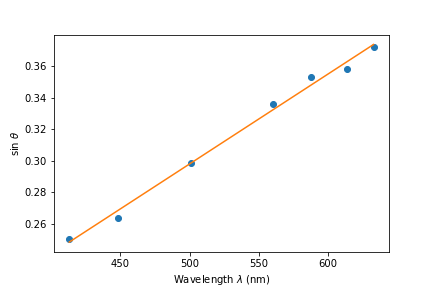
\includegraphics[scale = 0.55]{Figures/plot-1.png}
        \caption{The plot of $\lambda \sim \sin \theta$.\\ The values are imported from table (\ref{tab:data1}).}
        \label{fig:plot-1}
    \end{figure}
    From equation (\ref{eq7}), we have
    \begin{equation}
        \sin \theta = \dfrac{p}{g} \lambda
    \end{equation}
    As the spectral lines were obtained for the first order of diffraction, we have, $p = 1$.
    This implies the slope of $\lambda$ versus $\sin \theta$ curve will yield the value of $g$.
    \par
    The five summations of for the data set plotted in figure (\ref{fig:plot-1}) are as follows:
    \par
    \vspace{0.5cm}
    $S_{x} = \mathlarger{\mathlarger{\sum}} x_{i} = \SI{3757}{\nano \metre}$, \hspace{0.5cm} $S_{y} = \mathlarger{\mathlarger{\sum}} y_{i} = 2.23156$,
    \par
    \vspace{0.5cm}
    $S_{xx} = \mathlarger{\mathlarger{\sum}} x_{i}^2 = \SI{2.06e6}{\nano \metre \squared}$,
    \par
    \vspace{0.5cm}
    $S_{yy} = \mathlarger{\mathlarger{\sum}} y_{i}^2 = 0.725$,
    \par
    \vspace{0.5cm}
    $S_{xy} = \mathlarger{\mathlarger{\sum}} x_{i}y_{i} = \SI{1.22e3}{\nano \metre}$.
    \par
    \vspace{0.5cm}
    Now the slope is given by,
        \begin{equation}
        \label{eq9}
            m = \dfrac{S S_{xy} - S_{x}S_{y}}{S S_{xx} - S_{x}^2} = \SI{5.70e-4}{\per \nano \metre}
        \end{equation}
    Therefore, we have
    \begin{equation}
    \label{eq10}
        \boxed{g = \dfrac{1}{m} = \SI{1.76e3}{\nano \metre}}
    \end{equation}
    Now, from here, we know the value of $g$ and we can use it to determine the wavelengths of the hydrogen spectral lines using equation (\ref{eq7}).
    \par
    The plot of $(1/m^2 - 1/n^2)$ versus $1/ \lambda$ is plotted deriving the data from table (\ref{tab:data2}) in figure (\ref{fig:plot-2}). From equation (\ref{eq4}), we have the slope of this plot as the Rydberg constant for hydrogen atom, $R_H$.
    \begin{figure}
        \centering
        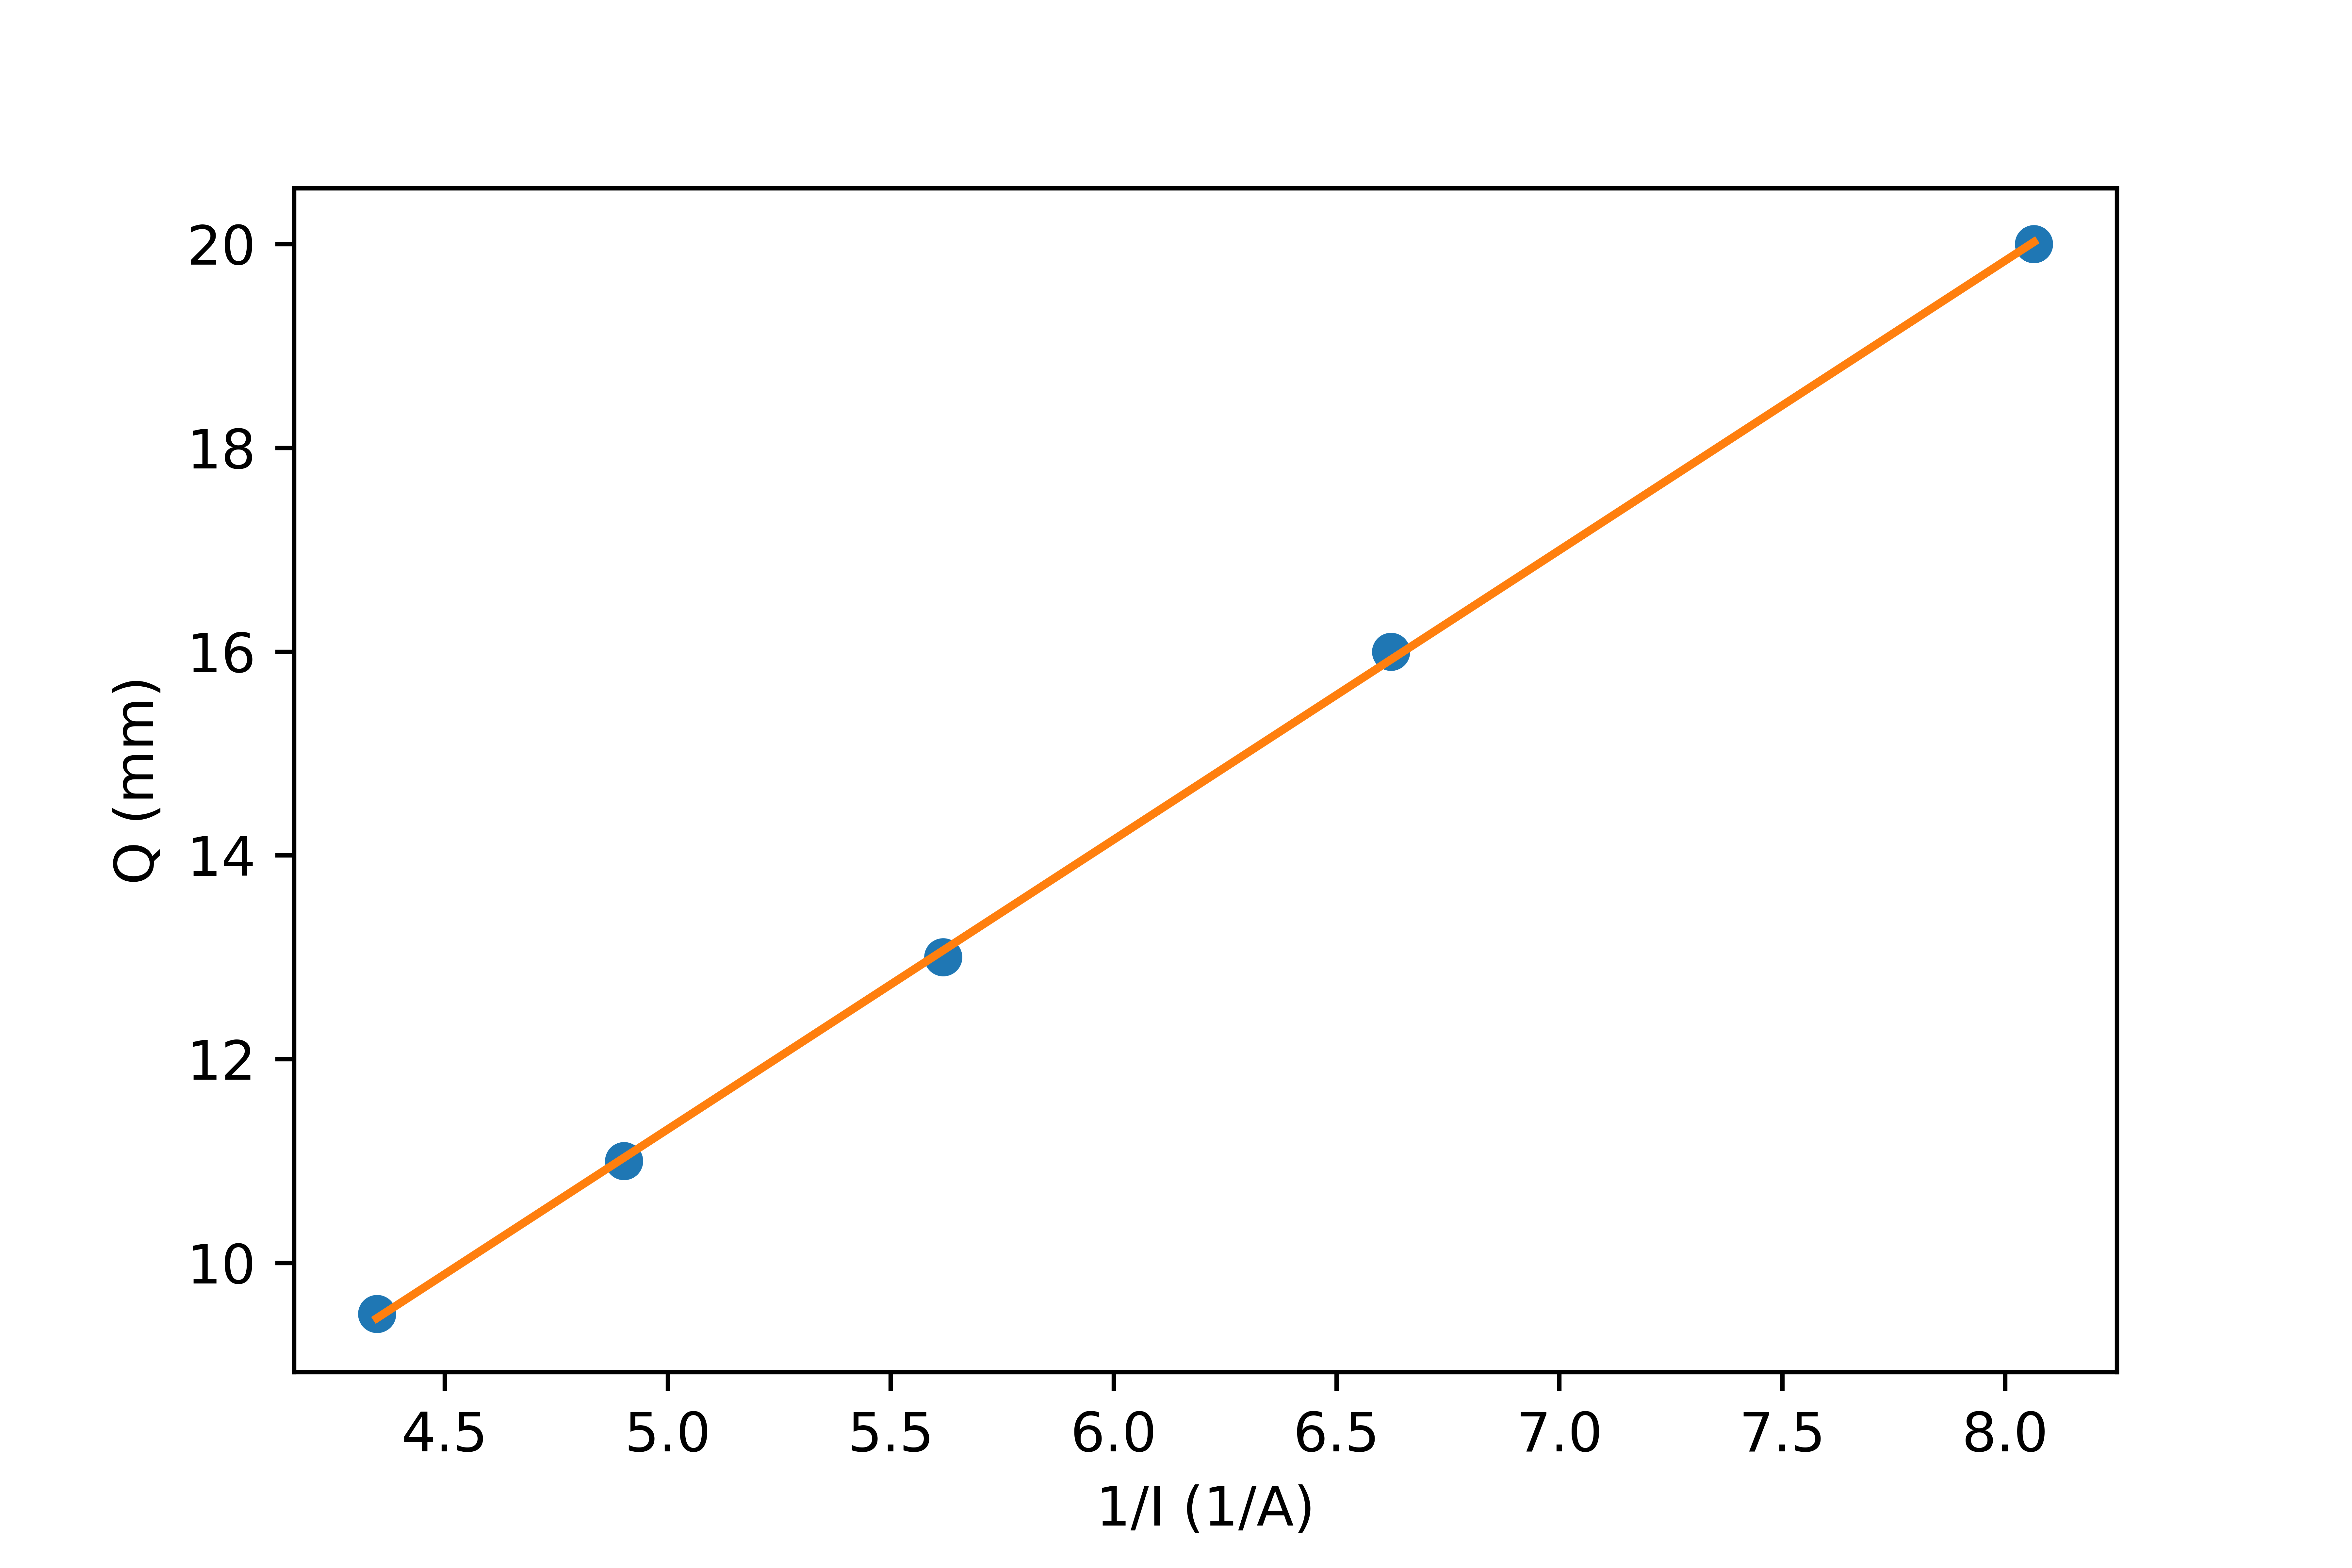
\includegraphics[scale = 0.75]{Figures/plot-2.png}
        \caption{The plot of $(1/m^2 - 1/n^2) \sim 1/ \lambda$.\\ The values are imported from table (\ref{tab:data2}). The labels represent the respective values of $m$ (the lower energy state) and $n$ (the higher energy state).}
        \label{fig:plot-2}
    \end{figure}
    \par
    The five summations for the data set plotted in figure (\ref{fig:plot-2}) are as follows:
    \par
    \vspace{0.5cm}
    $S_{x} = \mathlarger{\mathlarger{\sum}} x_{i} = 5.36 \times 10^{-1}$,
    \par
    \vspace{0.5cm}
    $S_{y} = \mathlarger{\mathlarger{\sum}} y_{i} = \SI{5.44e-3}{\per \nano \metre}$,
    \par
    \vspace{0.5cm}
    $S_{xx} = \mathlarger{\mathlarger{\sum}} x_{i}^2 = 9.85 \times 10^{-2}$,
    \par
    \vspace{0.5cm}
    $S_{yy} = \mathlarger{\mathlarger{\sum}} y_{i}^2 = \SI{1.03e-5}{\per \nano \metre \squared}$,
    \par
    \vspace{0.5cm}
    $S_{xy} = \mathlarger{\mathlarger{\sum}} x_{i}y_{i} = \SI{9.99e-4}{\per \nano \metre}$.
    \par
    \vspace{0.5cm}
    Now the slope is given by,
        \begin{equation}
        \label{eq11}
            m = \dfrac{S S_{xy} - S_{x}S_{y}}{S S_{xx} - S_{x}^2} = \SI{9.69e-3}{\per \nano \metre}
        \end{equation}
    That is, 
    \begin{equation}
        \boxed{R_H = \SI{0.969e7}{\metre}}
    \end{equation}
    
    


\section{Error Analysis}
We need to determine the uncertainty in the value of $R_H$. The error in $R_H$ comes from the error in slope in equation (\ref{eq11}). We know that the error in slope is given by,
\begin{equation}
\label{eq13}
    \sigma_m = \sigma_y \sqrt{\dfrac{S}{\Delta}}
\end{equation}
Here $\sigma_y$ is the uncertainty in values of $1/ \lambda$. The $1/ \lambda$ is calculated as
\begin{equation}
    \lambda = g \sin \theta
\end{equation}
Therefore, we need the uncertainties in $g$ and $\theta$ first. The uncertainty in $\sin \theta$ is given by,
\begin{equation}
    \Delta(\sin \theta) = (\cos \theta) \cdot \Delta \theta
\end{equation}
where $\Delta \theta$ is the least count of the spectrometer and is equal to $30''$ or $\SI{0.0001}{\radian}$, which can be approximated as the uncertainty in $\sin \theta$ itself. On the other hand the error in $g$ can be calculated from the error in slope in equation (\ref{eq9}) using equation (\ref{eq13}). For this, we have $\sigma_y = 0.0001$, number of terms $S = 7$ and $\Delta = S S_{xx} - S_{x}^2 = \SI{3.05e-13}{\metre}$. Putting the values in equation (\ref{eq13}), we get, 
\begin{equation}
    \sigma_m \approx \SI{479}{\per \metre}
\end{equation}
Now, percentage error in $m$ and $g$ would be same. The percentage error in $m$ is around 0.5\%. Therefore error in $g$ is given by 
\begin{equation}
    \sigma_g = \SI{0.01}{\micro \metre}
\end{equation}
Now we can move to the errors in hydrogen spectral lines and finally the error in $R_H$. Starting with the H-$\alpha$ line, the error is given by
\begin{equation}
    \sigma_{H-\alpha} = \sqrt{\Bigg(\dfrac{\partial \lambda}{\partial g}\sigma_g \Bigg)^2 + \Bigg(\dfrac{\partial \lambda}{\partial (\sin \theta)}\sigma_{\sin \theta} \Bigg)^2}
\end{equation}
After solving this, we get $\sigma_{H-\alpha} \approx \SI{4}{\nano \metre}$. Similarly we can solve for all spectra lines. Upon doing so, the errors are $\sigma_{H-\beta} \approx \SI{3}{\nano \metre}$ and $\sigma_{H-\gamma} \approx \SI{3}{\nano \metre}$.
\par
Finally for error in $R_H$, we have the error in slope as from equation (\ref{eq13}). For the error in values on $y$-axis (or $1/\lambda$), we will follow the same rule of same percentage error. Therefore, as the error in $\lambda$ are already found as are around 0.6\% of wavelengths, we have, the uncertainty in $1/\lambda$ as around \SI{1000}{\per \metre}.
From here, we can, suing equation (\ref{eq13}), calculate $\sigma_{R_H} = \SI{318}{\per \metre}$.
\section{Conclusions}
\begin{enumerate}
    \item The value of grating constant is $g = \SI{1.76\pm0.01}{\micro \metre}$.
    \item The wavelength values for the Hydrogen emission lines are as follows; \\
    \textbf{$H_{\alpha}$ = 706 $\pm$ 4 nm , $H_{\beta}$ = 528 $\pm$ 3 nm , $H_{\gamma}$ = 468 $\pm$ 3 nm}. \\
    Where, $\alpha$, $\beta$, $\gamma$ are the indices that represent the electronic de-excitation to n = 2 from m = 3,4,5 respectively.
    \item The value of Rydberg's constant is $R_H = (0.9693 \pm 0.0003) \times 10^7$ $m^{-1}$.
    \item The difference between the wavelengths of successive emission lines was decreasing as is seen from the graph. This means that the energy difference decreases too as \textbf{m} increases.
    \item The calculated value of Rydberg's constant is quite close to the literature value. Hence, we can say that the equation (\ref{eq4}) is verified experimentally.
    \item The values of $\theta$ on the left and right side are not completely identical, this could be due to improper alignment of the grating element, damage to it or due to manual errors in reading. This could be a source of error.
    \item The Hydrogen emission lines were observed and studied by measuring their wavelengths. The data was then used to find out the Rydberg's constant which was close to the expected value. The experiment was thus a success.
\end{enumerate}

\section{Precautions}
\begin{enumerate}
    \item Turn off the apparatus when not in use.
    \item Do not touch the grating element, with fingers. Make sure it is clean and aligned.
    \item Do not change the positions of the spectrometer and the spectral tube throughout
    the experiment.
    \item Do not look directly into the spectral tubes.
\end{enumerate}




% Produces the bibliography via BibTeX.

\end{document}
%
% ****** End of file apssamp.tex ******
